%%15:5:10 14/5/2017 -VieTeX creates E:\tex\book-mau\mau-dethi33\dethamkhao2017-toan.tex
\documentclass[12pt]{article}
\usepackage{amsmath,amsxtra,amssymb,latexsym, amscd,amsthm}
\usepackage{graphicx}
\usepackage{picinpar} %gói đưa hình vào bên cạnh
\usepackage{tikz} %Gói đưa hình vẽ bằng Geogebra vào
\usetikzlibrary{arrows}
\usepackage{tkz-tab}
\usepackage[utf8]{vietnam}
\usepackage{longtable}%
\usepackage{multicol}%
\usepackage{color}
\usepackage{shortlst}
\usepackage{enumerate}
\usepackage{mathpazo}
\usepackage[bookmarksnumbered, colorlinks,hyperindex, unicode]{hyperref}%
\voffset=-3cm
% \hoffset=-2cm
\textheight 25truecm
\textwidth 18.5truecm
\usepackage[baitap]{dethi} %Gói lệnh đề thi
\usepackage{titledot} %Làm mục lục tiếng việt
\usepackage{centerpage} %Quy trang vào tâm
\usepackage{lastpage}

\khoanh{\cboxv}
\daungoac{\cboxx}{}
\chuphuongan{\small\bfseries\Alph}
\mauchu{blue}
\PSNrandseed{\time}
\graphicspath{{hinh-cauhoi/}{images/}}
\def\v#1{\overrightarrow{#1}}
\tentruong{BỘ GIÁO DỤC VÀ ĐÀO TẠO}
\tenkhoa{ĐỀ THAM KHẢO}
\loaidethi{(Đề gồm  0\pageref{LastPage} trang)}%{ĐỀ THI LẠI}%%{ĐỀ CHÍNH THỨC}
\tenkythi{KỲ THI TRUNG HỌC PHỔ THÔNG QUỐC GIA 2017}
\tenmonhoc{Bài thi: TOÁN}
\madethi{003}
\tieudeduoi
\thoigian{\underline{Thời gian làm bài: 90 phút, không kể thời gian phát đề}}   
\hovaten{Họ và tên}         %Nếu không muốn có dòng này không gõ lệnh
\tenlop{Tên lớp}         %Nếu không muốn có dòng này không gõ lệnh
%\sobaodanh{Số báo danh}  %Nếu không muốn có dòng này không gõ lệnh
\graphicspath{{dethamkhao/}}
\renewcommand{\bonpa}[4]{#1#2#3#4}
\setlength{\baselineskip}{11truept}
\begin{document}
\soanthao

\title{\bf TRỢ GIÚP [BAITAP] ĐẦU VÀO  DETHI.STY 3.3} % Ten bai
\author{{\bf Nguyễn Hữu Điển}\\
Khoa Toán - Cơ - Tin học\\
ĐHKHTN Hà Nội, ĐHQGHN
} % Tac gia
\date{} % Ngay

\maketitle
%%15:15:57 14/5/2017 -VieTeX creates E:\tex\book-mau\mau-dethi33\vd13-cauhoi-detk2917-toan.tex
 
\baitracnghiem{detk2017:b01}{
Cho hàm số
$y=x^3-3x$ có đồ thị (C). Tìm số giao điểm của (C) và trục hoành.
}{ 
\datcot\bonpa
{\sai{2.}}
{\dung{3.}}
{\sai{1.}}
{\sai{0.}}
\loigiai{
Ta có $y=0 \Leftrightarrow x^3-3x=0\Leftrightarrow x=0, x=\pm \sqrt3$.
Do đó số giao điểm  $(C)$ và trục hoành là  3 .
}
} 

  
\baitracnghiem{detk2017:b02}{
 Tìm đạo hàm của hàm số  $y=\log x$.
}{ 
\datcot[2]\bonpa
{\sai{$y'=\dfrac{1}{x}$.}}
{\sai{$y'=\dfrac{\ln10}{x}$.}}
{\dung{$y'=\dfrac{1}{x\ln10}$.}}
{\sai{$y'=\dfrac{1}{10\ln x}$.}}
\loigiai{
$y=\log x\Rightarrow y'=(\log x)'=\dfrac{1}{x\ln 10}$.
}
} 
 
  
\baitracnghiem{detk2017:b03}{
  Tìm tập nghiệm  $S$ của bất phương trình $5^{x+1}-\dfrac{1}{5}>0$.
}{ 
\datcot[2]\bonpa
{\sai{$S=(1;+\infty)$.}}
{\sai{$S=(-1;+\infty)$.}}
{\dung{$S=(-2;+\infty)$.}}
{\sai{$S=(-\infty,-2)$.}}
\loigiai{
Ta có $5^{x+1}-\dfrac{1}{5}>0\Leftrightarrow 5^{x+1}>5^{-1}\Leftrightarrow x+1>-1\Leftrightarrow x>-2$.
}
} 
 
  
\baitracnghiem{detk2017:b04}{
Kí hiệu  $a, b$ lần lượt là phần thực và phần ảo của số phức $3-2\sqrt2 i$. Tìm $a,b$.
}{ 
\datcot\bonpa
{\sai{$a=3;b=2$.}}
{\sai{$a=3;b=2\sqrt2$.}}
{\sai{$a=3;b=\sqrt2$.}}
{\dung{$a=3;b=-2\sqrt2$.}}
\loigiai{
$z=3-2\sqrt2 i$ có phần thực là  $3$ và phần ảo là  $-2\sqrt2$.
}
} 

  
\baitracnghiem{detk2017:b05}{
 Tính môđun của số phức $z$ biết  $\bar z=(4-3i)(1+i)$.
}{ 
\datcot\bonpa
{\sai{$|z|=25\sqrt2$.}}
{\sai{$|z|=7\sqrt2$.}}
{\dung{$|z|=5\sqrt2$.}}
{\sai{$|z|=\sqrt2$.}}
\loigiai{
Ta có $\bar z=(4-3i)(1+i)=7+i\Rightarrow z=7-i$.
Do đó $|z|=\sqrt{7^2+(-1)^2}=5\sqrt2$.
}
} 

  
\baitracnghiem{detk2017:b06}{
Cho hàm số $y=\dfrac{x-2}{x+1}$. Mệnh đề nào dưới đây đúng?
}{ 
\datcot[2]\bonpa
{\sai{Hàm số nghịch biến trên khoảng $(-\infty;-1)$.}}
{\dung{Hàm số đồng biến trên khoảng $(-\infty;-1)$.}}
{\sai{Hàm số đồng biến trên khoảng $(-\infty;+\infty)$.}}
{\sai{Hàm số nghịch biến trên khoảng $(-1;+\infty)$.}}
\loigiai{
$y'=\dfrac{3}{(x+1)^2}>0 \forall x\in \mathbb{R}$ nên hàm số đã cho đồng biến trên các khoảng $(-\infty;-1);(-1;+\infty)$
}
} 

  
\baitracnghiem{detk2017:b07}{
 Cho hàm số $y=f(x)$ có bảng biến thiên
\begin{window}[0,r,{\hspace*{2cm}
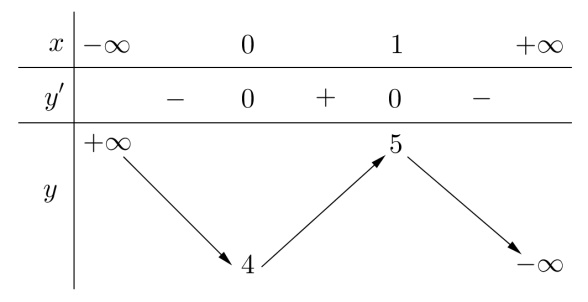
\includegraphics[scale=0.55]{dethamkhao01}},]
như hình vẽ bên. Mệnh đề nào dưới đây đúng ?
\end{window}
\vspace*{0.5cm}
}{
\datcot[2]\bonpa
{\dung{$y_{\mbox{CĐ}}=5$.}}
{\sai{$y_{\mbox{CT}}=0$.}}
{\sai{$\min\limits_{\mathbb{R}} y=4$.}}
{\sai{$\max\limits_{\mathbb{R}} y=5$.}}
\loigiai{
Dựa vào bảng biến thiên ta suy ra $y_{\mbox{CĐ}}=5$.
}
} 
 
  
\baitracnghiem{detk2017:b08}{
 Trong không gian với hệ tọa độ, $Oxyz$ tìm tọa độ tâm $I$ và bán kính $R$ của mặt cầu\\
$(x-1)^2+(y+2)^2+(z-4)^2=20$.
}{ 
\datcot[2]\bonpa
{\sai{$I(-1;2;-4),R=5\sqrt2$.}}
{\sai{$I(-1;2;-4),R=2\sqrt5$.}}
{\sai{$I(-1;2;-4),R=20$.}}
{\dung{$I(1;-2;4),R=2\sqrt5$.}}
\loigiai{
Mặt cầu
$(x-1)^2+(y+2)^2+(z-4)^2=20$ có tâm $I(1;-2;4)$, bán kính $R=2\sqrt5$.
}
} 

  
\baitracnghiem{detk2017:b09}{
 Trong không gian với hệ tọa độ  , $Oxyz$ phương trình nào dưới đây là phương trình chính tắc của
đường thẳng $d:\begin{cases}
x=1+2t&\\
y=3t&\\
z=-2+t&
\end{cases}$?
}{ 
\datcot[2]\bonpa
{\sai{$\dfrac{x+1}{2}=\dfrac{y}{3}=\dfrac{z-2}{1}$.}}
{\sai{$\dfrac{x-1}{1}=\dfrac{y}{3}=\dfrac{z+2}{-2}$.}}
{\sai{$\dfrac{x+1}{1}=\dfrac{y}{3}=\dfrac{z-2}{-2}$.}}
{\dung{$\dfrac{x-1}{2}=\dfrac{y}{3}=\dfrac{z+2}{1}$.}}
\loigiai{
Dựa vào phương trình tham số ta suy ra  $d$ qua  $A(1;0;-2)$ và có vtcp  $\vec{u}(2;3;1)$  nên suy
ra  $d$ có phương trình chính tắc là $\dfrac{x-1}{2}=\dfrac{y}{3}=\dfrac{z+2}{1}$.
} 
} 

  
\baitracnghiem{detk2017:b10}{
 Tìm nguyên hàm của hàm số
$f(x)=x^2+\dfrac{2}{x^2}$.
}{ 
\datcot[2]\bonpa
{\dung{$\int f(x)dx=\dfrac{x^3}{3}-\dfrac{2}{x}+C$.}}
{\sai{$\int f(x)dx=\dfrac{x^3}{3}-\dfrac{1}{x}+C$.}}
{\sai{$\int f(x)dx=\dfrac{x^3}{3}+\dfrac{2}{x}+C$.}}
{\sai{$\int f(x)dx=\dfrac{x^3}{3}+\dfrac{1}{x}+C$.}}
\loigiai{
Ta có $\int\left(x^2+\dfrac{2}{x^2}\right)dx=\dfrac{x^3}{3}-\dfrac{2}{x}+C$.
}
} 
 
  
\baitracnghiem{detk2017:b11}{
 Cho hàm số  $y=f(x)$ có bảng biến thiên như hình vẽ dưới đây. Hỏi đồ thị của hàm số đã cho có
bao nhiêu đường tiệm cận?
\begin{center}
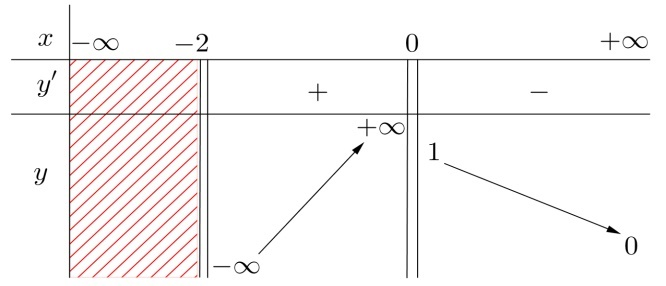
\includegraphics[scale=0.6]{detk11}
\end{center}
}{ 
\datcot\bonpa
{\sai{$1$.}}
{\dung{$3$.}}
{\sai{$2$.}}
{\sai{$4$.}}
\loigiai{
$\lim\limits_{x\rightarrow 2^+}y=-\infty$ nên $x=-2$ là TCĐ.
$\lim\limits_{x\rightarrow 0}y=+\infty$ nên $x=0$ là TCĐ.
$\lim\limits_{x\rightarrow +\infty}y=0$ nên $y=0$ là TCN.
}
} 
 
  
\baitracnghiem{detk2017:b12}{
 Tính giá trị của biểu thức $P=\left(7+4\sqrt3\right)^{2017}\left(4\sqrt3-7\right)^{2016}$
}{ 
\datcot\bonpa
{\sai{$P=1$.}}
{\sai{$P=7-4\sqrt3$.}}
{\dung{$P=7+4\sqrt3$.}}
{\sai{$P=\left(7+4\sqrt3\right)^{2016}$.}}
\loigiai{{\allowdisplaybreaks 
\begin{align*}
\left(7+4\sqrt3\right)^{2017}\left(4\sqrt3-7\right)^{2016}&=\left(7+4\sqrt3\right)\left(7+4\sqrt3\right)^{2016}\left(4\sqrt3-7\right)^{2016}\\ 
&=\left(7+4\sqrt3\right)\left[\left(2+\sqrt3\right)^2\right]^{2016}\left(4\sqrt3-7\right)^{2016}\\ 
&=\left(7+4\sqrt3\right)\left[\left(2+\sqrt3\right)^2\right]^{2016}\left[-\left(2-\sqrt3\right)^2\right]^{2016}\\
&=\left(7+4\sqrt3\right)\left[-\left(2+\sqrt3\right)^2\left(2-\sqrt3\right)^2\right]^{2016}\\
&=\left(7+4\sqrt3\right).1=\left(7+4\sqrt3\right).
\end{align*}
}
}
} 
 
  
\baitracnghiem{detk2017:b13}{
 Cho  $a$ là số thực dương,  $a\ne 1$ và $P=\log_{\sqrt[3]{a}}a^3$. Mệnh đề nào dưới đây đúng?
}{ 
\datcot\bonpa
{\sai{$P=3$.}}
{\sai{$P=1$.}}
{\dung{$P=9$.}}
{\sai{$P=\dfrac{1}{3}$.}}
\loigiai{
Ta có $\log_{\sqrt[3]{a}}a^3=\log_{a^{\frac{1}{3}}}a^3=9\log_a a=9$.
}
} 

  
\baitracnghiem{detk2017:b14}{
 Hàm số nào dưới đây đồng biến trên khoảng $(-\infty;+\infty)$?
}{ 
\datcot\bonpa
{\dung{$y=3x^3+3x-2$.}}
{\sai{$y=2x^3-5x+1$.}}
{\sai{$y=x^4+3x^2$.}}
{\sai{$y=\dfrac{x-2}{x+1}$.}}
\loigiai{
Ta có $y'>0\quad \forall x\in R$, $(3x^3+3x-2)'=9x^2+3>0, \forall x\in R$.
}
} 
 
  
\baitracnghiem{detk2017:b15}{
  Cho hàm số  $f(x)=x\ln x$ Một trong bốn đồ thị cho trong bốn phương án A, B, C, D dưới đây là
đồ thị của hàm số  $y=f'(x)$. Tìm đồ thị đó.
}{ 
\datcot\bonpa
{\sai{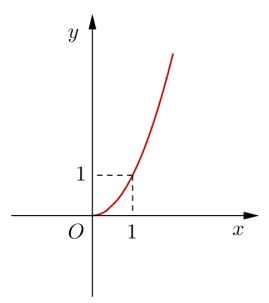
\includegraphics[scale=0.5]{detk15a}}}
{\sai{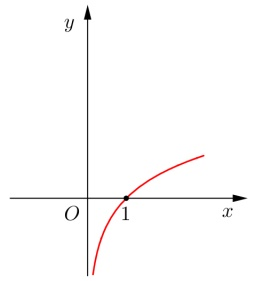
\includegraphics[scale=0.5]{detk15b}}}
{\dung{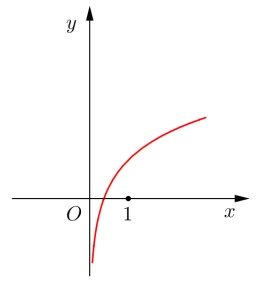
\includegraphics[scale=0.5]{detk15c}}}
{\sai{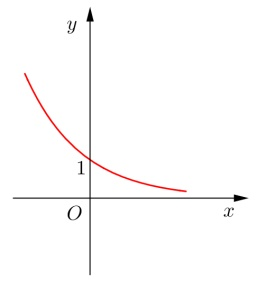
\includegraphics[scale=0.5]{detk15d}}}
\loigiai{
Ta có $f'(x)=(x\ln x)'=\ln x+1, \forall x>0. f'(1)=1$.
Hàm số  $f'(x)=\ln x+1, x\ne 0$ có điều kiện $x>0$, nên loại đáp án A và D.
Hàm số cắt trục hoành tại điểm có hoành độ $x=\dfrac{1}{e}<1$
nên loại B.\\
Đồ thị hàm số $f'(x)=\ln x+1$ là 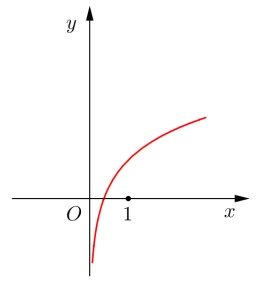
\includegraphics[scale=0.5]{detk15c}.
}
} 

  
\baitracnghiem{detk2017:b16}{
 Tính thể tích $V$ của khối lăng trụ tam giác đều có tất cả các cạnh bằng $a$.
}{ 
\datcot\bonpa
{\sai{$V=\dfrac{a^3\sqrt3}{6}$.}}
{\sai{$V=\dfrac{a^3\sqrt3}{12}$.}}
{\sai{$V=\dfrac{a^3\sqrt3}{2}$.}}
{\dung{$V=\dfrac{a^3\sqrt3}{4}$.}}
\loigiai{
% \begin{window}[0,r,{\hspace*{0.5cm}
% 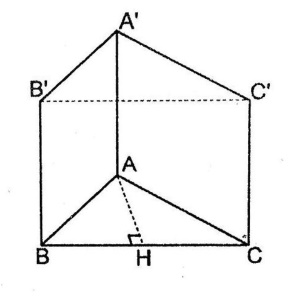
\includegraphics[scale=0.5]{detkl16}\hspace*{2cm}},{\label{fig:detkl16}}]
% \begin{minipage}[b]{\textwidth/2-1em}
Khối lăng trụ tam giác đều có chiều cao  $h=a$ và
diện tích đá $S=\dfrac{1}{2}AH.BC=\dfrac{1}{2}\dfrac{a\sqrt3}{2}.a=\dfrac{a^2\sqrt3}{4}$. 
Vậy $V=S.h=\dfrac{a^2\sqrt3}{4}$.
% \end{minipage}
% \begin{minipage}[b]{\textwidth/2-1em}
% \centering
\begin{center}
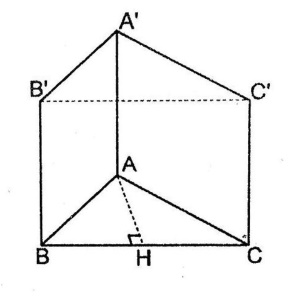
\includegraphics[scale=0.7]{detkl16}
\end{center}
% \end{minipage}
%\end{window}
}
} 

  
\baitracnghiem{detk2017:b17}{
 Trong không gian với hệ tọa độ $Oxyz$ cho các điểm  $A(3;-4;0), B(-1;1;3)$ và  $C(3;1;0).$ Tìm tọa
độ điểm  $D$ trên trục hoành sao cho  $AD=BC$.  
}{ 
\datcot[2]\bonpa
{\sai{$D(-2;0;0)$ hoặc $D(-4;0;0)$.}}
{\sai{$D(0;0;0)$ hoặc $D(-6;0;0)$.}}
{\sai{$D(6;0;0)$ hoặc $D(12;0;0)$.}}
{\dung{$D(0;0;0)$ hoặc $D(6;0;0)$.}}
\loigiai{
Ta có $D\in Ox$ nên $D(a;0;0)$. Mặt khác $AD=BC$ hay $\sqrt{(a-3)^2+(-4)^2}=\sqrt{3^2+4^2} \Leftrightarrow \left[\begin{matrix}
a=6\\ 
a=0\\ 
\end{matrix}\right.$
}
} 
 
  
\baitracnghiem{detk2017:b18}{
 Kí hiệu $z_1$ và $z_2$ là hai nghiệm phức của phương trình $z^2+z+1=0$. Tính $P=z_1^2+z_2^2+z_1z_2$.
}{ 
\datcot\bonpa
{\sai{$P=1$.}}
{\sai{$P=2$.}}
{\sai{$P=-1$.}}
{\dung{$P=0$.}}
\loigiai{
Theo Viet, ta có $\begin{cases}
z_1+z_2&=-1\\
z_1.z_2&=1.
\end{cases}$ Do đó $P=z_1^2+z_2^2+z_1z_2=(z_1+z_2)^2-z_1z_2=0$.
}
} 

  
\baitracnghiem{detk2017:b19}{
Tính giá trị nhỏ nhất của hàm số $y=3x+\dfrac{4}{x^2}$ trên khoảng $(0;+\infty)$.
}{ 
\datcot\bonpa
{\dung{$\min\limits_{(0;+\infty)}y=3\sqrt[3]{9}$.}}
{\sai{$\min\limits_{(0;+\infty)}y=7$.}}
{\sai{$\min\limits_{(0;+\infty)}y=\dfrac{33}{5}$.}}
{\sai{$\min\limits_{(0;+\infty)}y=2\sqrt[3]{9}$.}}
\loigiai{
Ta có $y'=3-\dfrac{8}{x^2}$. $y'=0\Leftrightarrow3-\dfrac{8}{x^3}
\Leftrightarrow x=\dfrac{2}{\sqrt[3]{3}}
\Rightarrow y=\dfrac{9}{\sqrt[3]{3}}=3\sqrt[3]{9}$. Bảng biến thiên
\begin{center}
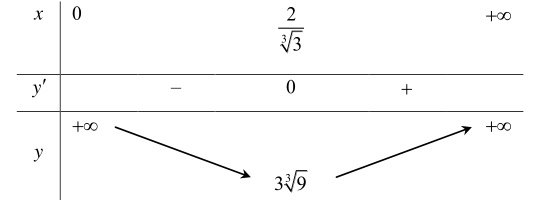
\includegraphics[scale=0.7]{detkl19}
\end{center}
Vậy $\min\limits_{(0;+\infty)}y=3\sqrt[3]{9}$.
}
} 
 
  
\baitracnghiem{detk2017:b20}{
 Hình đa diện trong hình vẽ bên có bao nhiêu mặt?
\begin{window}[0,r,{\hspace*{1cm}
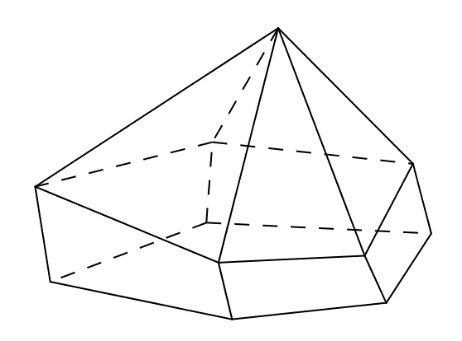
\includegraphics[scale=0.35]{detk20}\hspace*{2cm}},]
\quad\phantom{A}
\end{window}
% \vspace*{-0.5cm}
}{ 
\datcot[2]\bonpa
{\sai{$6$.}}
{\sai{$10$.}}
{\sai{$12$.}}
{\dung{$11$.}}
\loigiai{
Đếm được 11 mặt.
(Chú ý ta có thể dò lại nhờ định lý Euler Đ + M = C + 2).
}
} 
 
  
\baitracnghiem{detk2017:b21}{
  Gọi $S$ là diện tích hình phẳng $(H)$ giới hạn bởi các
\begin{window}[0,r,{\hspace*{2cm}
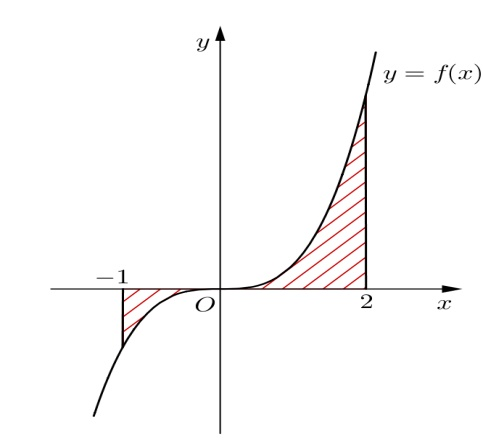
\includegraphics[scale=0.45]{detk21}\hspace*{1cm}},]
đường  $y=f(x)$ trục hoành và hai đường thẳng  $x=-1,x=-2$
(như hình vẽ bên). Đặt $a=\int_{-1}^0f(x)dx, b=\int_0^2f(x)dx$,mệnh đề
nào dưới đây đúng?
\end{window}
\vspace*{0.3cm}
}{
\datcot[2]\bonpa
{\dung{$S=b-a$.}}
{\sai{$S=b+a$.}}
{\sai{$S=-b+a$.}}
{\sai{$S=-b-a$.}}
\loigiai{
Ta có $S=\int_{-1}^0|f(x)|dx+\int_0^2|f(x)|dx=-a+b=b-a$.
}
} 

  
\baitracnghiem{detk2017:b22}{
 Tìm tập nghiệm  $S $ của phương trình $\log_2(x-1)+\log_2(x+1)=3$.
}{ 
\datcot\bonpa
{\sai{$S=\{-3;3\}$.}}
{\sai{$S=\{4\}$.}}
{\dung{$S=\{3\}$.}}
{\sai{$S=\{-\sqrt{10};\sqrt{10}\}$.}}
\loigiai{
Điều kiện: $x\ge 1$. Ta có: $\log_2(x-1)+\log_2(x+1)=3\Rightarrow\log_2(x^2-1)=3.$
$\Rightarrow x^2-1=2^3\Rightarrow \left|\begin{matrix}
x=3\\ 
x=-3\\ 
\end{matrix}\right.$. Đối chiếu điều kiện, ta được $x=3$.
}
} 
 
  
\baitracnghiem{detk2017:b23}{
 Đường cong trong hình vẽ bên là đồ thị của một hàm số 
\begin{window}[0,r,{\hspace*{1cm}
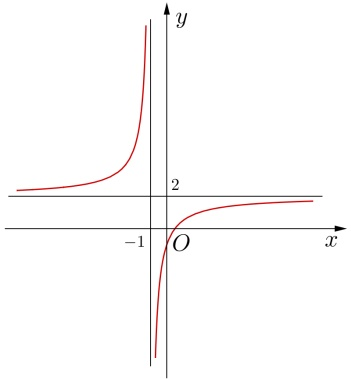
\includegraphics[scale=0.5]{detk23}\hspace*{0.5cm}},]
trong bốn
hàm số được liệt kê ở bốn phương án A, B, C, D dưới đây. Hỏi đó là hàm
số nào?
\end{window}
\vspace*{0.5cm}
}{ 
\datcot[2]\bonpa
{\sai{$y=\dfrac{2x+3}{x+1}$.}}
{\dung{$y=\dfrac{2x-1}{x+1}$.}}
{\sai{$y=\dfrac{2x-2}{x-1}$.}}
{\sai{$y=\dfrac{2x+1}{x-1}$.}}
\loigiai{
Tiệm cận đứng  $x=-1$.
Tiệm cận ngang  $y=2$. Không đi qua điểm $A\left(\dfrac{1}{2},0\right)$.
Loại \dapansai.\\
Đồ thị hàm số có dạng của hàm số đồng biến nên chọn \dapandung.\\
Hoặc ta có thể xét đồ thị đi qua điểm $A\left(\dfrac{1}{2},0\right)$ nên chọn  \dapandung.
}
} 
 
  
\baitracnghiem{detk2017:b24}{
 Tính tích phân $I=\int_1^22x\sqrt{x^2-1}dx$ bằng cách đặt $u=x^2-1$, mệnh đề nào dưới đây đúng?
}{ 
\datcot\bonpa
{\sai{$I=2\int_0^3\sqrt{u}du$.}}
{\sai{$I=\int_1^2\sqrt{u}du$.}}
{\dung{$I=\int_0^3\sqrt{u}du$.}}
{\sai{$I=\dfrac{1}{2}\int_1^2\sqrt{u}du$.}}
\loigiai{
Đặt $u=x^2-1, du=2xdx$. Đối cận $\begin{tabular}{| l | l |}
\hline
x-1&u=0\\
\hline 
x=2&u=3\\
\hline 
\end{tabular}$.
Vậy $I=\int_0^3\sqrt{u}du$.
}
} 
 
  
\baitracnghiem{detk2017:b25}{
 Trên mặt phẳng tọa độ, điểm $M $ là điểm biểu diễn 
\begin{window}[0,r,{\hspace*{1cm}
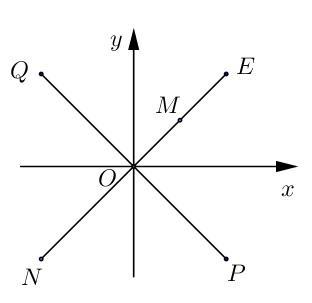
\includegraphics[scale=0.5]{detk25}\hspace*{0.5cm}},]
của số phức $z$
(như hình vẽ bên). Điểm nào trong hình vẽ là điểm biểu diễn của số phức $2z$?
\end{window}
}{ 
\datcot[2]\bonpa
{\sai{Điểm $N$.}}
{\sai{Điểm $Q$.}}
{\dung{Điểm $E$.}}
{\sai{Điểm $P$.}}
\loigiai{
Xét  $M(a,b)$ biểu diễn số phức  $z=a+bi (a,b\in R)$ trên mặt phẳng phức $Oxy$.
Vậy $E(2a,2b)$ biểu diễn số phức  $2z=2a+2bi (a,b\in R)$ trên mặt phẳng phức $Oxy$.
}
} 
 
  
\baitracnghiem{detk2017:b26}{
 Cho hình nón có diện tích xung quanh bằng $3\pi a^2$ và bán kính đáy bằng $a$. Tính độ dài đường sinh $l$
của hình nón đã cho.
}{ 
\datcot\bonpa
{\sai{$l=\dfrac{\sqrt5a}{2}$.}}
{\sai{$l=2\sqrt2 a$.}}
{\sai{$l=\dfrac{3a}{2}$.}}
{\dung{$l=3a$.}}
\loigiai{
$S_{xq}=\pi R I\Rightarrow l=\dfrac{S_{xq}}{\pi R}=\dfrac{3\pi a^2}{\pi a}=3a$.
}
} 
 
  
\baitracnghiem{detk2017:b27}{
 Cho $\int\limits_0^1\dfrac{dx}{e^x+1}=a+b\ln\dfrac{1+e}{2}$, với $a,b$ là các số hữu tỉ. Tính $S=a^3+b^3$.
}{ 
\datcot\bonpa
{\sai{$S=2$.}}
{\sai{$S=-2$.}}
{\dung{$S=0$.}}
{\sai{$S=1$.}}
\loigiai{
$\int_{0}^1\dfrac{1}{e^x+1}dx=\int_0^1\dfrac{e^x}{(e^x+1)e^x}dx$. Đặt $t=e^x\Rightarrow dt=e^x dx$,\\
$I=\int_1^e\dfrac{1}{t(t+1)}dt=\int_1^e\left(\dfrac{1}{t}-\dfrac{1}{t+1}\right)dt=\ln\left.\left|\dfrac{t}{t+1}\right|\right|^e_1=1-\ln\dfrac{e+1}{2}$. Khi đó $a=1, b=-1$ suy ra $S=0$.
}
} 

  
\baitracnghiem{detk2017:b28}{
 Tính thể tích $V $ của khối trụ ngoại tiếp hình lập phương có cạnh bằng $a$.
}{ 
\datcot\bonpa
{\sai{$V=\dfrac{\pi a^3}{4}$.}}
{\sai{$V=\pi a^3$.}}
{\sai{$V=\dfrac{\pi a^3}{6}$.}}
{\dung{$V=\dfrac{\pi a^3}{2}$.}}
\loigiai{
$V=Bh=\pi R^2 h=\pi\left(\dfrac{\sqrt2}{2}\right)^2a=\pi\dfrac{a^3}{2}$.
}
} 
 
\baitracnghiem{detk2017:b29}{
 Trong không gian với hệ tọa độ $Oxyz$, cho mặt cầu $(S)$ có tâm  $ I(3;2;-1)$ và đi qua điểm $A(2;1;2)$.
Mặt phẳng nào dưới đây tiếp xúc với $(S)$ tại $A$?
}{ 
\datcot\bonpa
{\sai{$x+y-3z-8=0$.}}
{\sai{$x-y-3z+3=0$.}}
{\sai{$x+y+3z-9=0$.}}
{\dung{$x+y-3z+3=0$.}}
\loigiai{
$\overrightarrow{IA}=(-1;-1;3)$ suy ra mặt phẳng đi qua  $A(2;1;2)$ và nhận  $\overrightarrow{IA}=(-1;-1;3)$ làm VTPT là:
$x+y-3z+3=0$.
}
} 

  
\baitracnghiem{detk2017:b30}{
 Trong không gian với hệ tọa độ  $Oxyz$, cho mặt phẳng  $(P): 2x-2y-z+1=0$ và đường thẳng
$\Delta:\dfrac{x-1}{2}=\dfrac{y+2}{1}=\dfrac{z-1}{2}$. Tính khoảng cách $d$ giữa $\Delta$ và $(P)$. 
}{ 
\datcot\bonpa
{\sai{$d=\dfrac{1}{3}$.}}
{\sai{$d=\dfrac{5}{3}$.}}
{\sai{$d=\dfrac{2}{3}$.}}
{\dung{$d=2$.}}
\loigiai{
Ta có véctơ pháp tuyến của mặt phẳng $(P): 2x-2y-z+1=0$ là $\overrightarrow{n_p}=(2;-2;1)$.\\
Véctơ chỉ phương của đường thẳng $\Delta:\dfrac{x-1}{2}=\dfrac{y+2}{1}=\dfrac{z-1}{2}$ là $\overrightarrow{u_{\Delta}}=(2;1;2)$.\\
Mà $\overrightarrow{n_p}.\overrightarrow{u_{\Delta}}=0$
nên $\Delta//(P)$. Vậy $d( (P);\Delta)=d(M_0;(P))$ với $M_0(1;-2;1)\in \Delta$. $d=\dfrac{|2.1-2.(-2)-1|}{\sqrt{2^2+(-2)^2+(-1)^2}}=\dfrac{6}{3}=2.$
}
} 

  
\baitracnghiem{detk2017:b31}{
 Tìm tất cả các giá trị thực của tham số $m $ để hàm số $y=(m-1)x^4-2(m-3)x^2+1$ \textbf{không} có cực đại.
}{ 
\datcot\bonpa
{\dung{$1\le m\le 3$.}}
{\sai{$ m\le 1$.}}
{\sai{$m\ge 1$.}}
{\sai{$1< m\le 3$.}}
\loigiai{
Ta có $y'=4(m-1)x^3-4(m-3)x=4x( (m-1)x^2-m+3)$.\\
Xét với $m=1\Rightarrow y=4x^2+1$ hàm số không có cực đại. Vậy  $m=1$ thỏa mãn (1).\\
Xét với  $m>1$ khi đó hàm số là hàm bậc 4 trùng phương với hệ số  $a>0$ để hàm số
không có cực đại thì  $y'=0$ chỉ có một nghiệm duy nhất  $x=0$.\\
Hay  $(m-1)x^2-m+3=0$  vô nghiệm $\Leftrightarrow x^2=\dfrac{m-3}{m-1}\le 0\Leftrightarrow 1<m\le 3$ (2).\\
Xét với  $m<1$ hàm số bậc 4 trùng phương có hệ số $a<0$ luôn có cực đại. (3)\\
Kết luận : Từ (1),(2),(3) ta có để hàm số không có cực đại thì $1\le m\le 3$.
}
} 
 
  
\baitracnghiem{detk2017:b32}{Hàm số $y=(x-2)(x^2-1)$ có đồ thị như hình vẽ bên.
\begin{window}[0,r,{\hspace*{1cm}
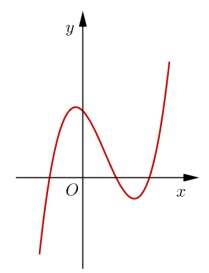
\includegraphics[scale=0.6]{detk32}\hspace*{0.5cm}},]
Hình nào
dưới đây là đồ thị của hàm số $y=|x-2|(x^2-1)$?
\end{window}
}{ 
 \setlength{\shortitemwidth}{\textwidth/6-3em}
% \datcot
\bonpa
{\dung{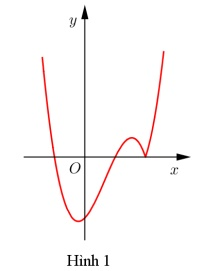
\includegraphics[scale=0.5]{detk32a} \\ Hình 1.}}
{\sai{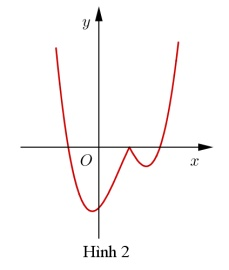
\includegraphics[scale=0.5]{detk32b} \\ Hình 2.}}
{\sai{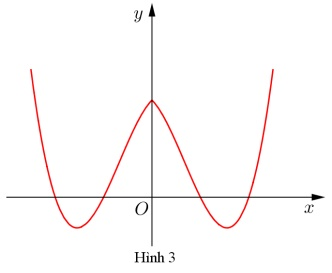
\includegraphics[scale=0.5]{detk32c} \\ Hình 3.}}
{\sai{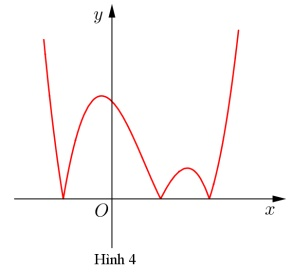
\includegraphics[scale=0.5]{detk32d} \\ Hình 4.}}
%  \setlength{\shortitemwidth}{\textwidth/4-3em}
\loigiai{
Đồ thị của hàm số $y=|x-2|(x^2-1)$ là 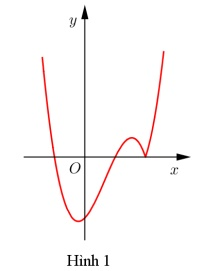
\includegraphics[scale=0.5]{detk32a}\\
Cách 2:
Hàm số $y=(x-2)(x^2-1)$ có bảng xét giấu là
\begin{center}
\begin{tabular}{| l | c  c  c  c  c  c  c  c  c |}
\hline
$x$&$-\infty$&&-1&&1&&2&&$+\infty$\\ 
\hline
$(x-2)$&&-&|&-&|&-&0&+&\\ 
\hline
$(x^2-1)$&&+&0&-&0&+&|&+&\\ 
\hline
$y$&&-&0&+&0&-&0&+&\\ 
\hline
\end{tabular}
\end{center}
%
Hàm số $y=|x-2|(x^2-1)$ có bảng xét dấu là 
\begin{center}
\begin{tabular}{| l | c  c  c  c  c  c  c  c  c |}
\hline
$x$&$-\infty$&&-1&&1&&2&&$+\infty$\\ 
\hline
$|x-2|$&&+&|&+&|&+&0&+&\\ 
\hline
$(x^2-1)$&&+&0&-&0&+&|&+&\\ 
\hline
$y$&&+&0&-&0&+&0&+&\\ 
\hline
\end{tabular}
\end{center}
Từ bảng xét dấu ta nhận xét đồ thị hàm số $y=|x-2|(x^2-1)$.\\
Trên các khoảng  $(-\infty;-1)$, $(-1;0)$ và  $(1;2)$ lấy đối xứng đồ thị hàm số $y=(x-2)(x^2-1)$.\\
Trên khoảng  $(2;+\infty)$ là đồ thị hàm số $y=(x-2)(x^2-1)$.
}
} 

  
\baitracnghiem{detk2017:b33}{
 Cho $a,b$ là các số thực dương thỏa mãn  $a\ne 1, a\ne \sqrt{b}$ và $\log_a b=\sqrt3$. Tính $P=\log_{\frac{\sqrt{b}}{a}}\sqrt{\dfrac{b}{a}}$
}{ 
\datcot\bonpa
{\sai{$P=-5+3\sqrt3$.}}
{\sai{$P=-1+\sqrt3$.}}
{\dung{$P=-1-\sqrt3$.}}
{\sai{$P=-5-3\sqrt3$.}}
\loigiai{
Ta có $\log_{\frac{\sqrt{b}}{a}}\sqrt{\dfrac{b}{a}}=\dfrac{1}{2}\dfrac{\log_ab-1}{\dfrac{1}{2}\log_ab-1}=\dfrac{\sqrt3-1}{\sqrt3-2}=-1-\sqrt3$.
}
} 
 
  
\baitracnghiem{detk2017:b34}{
 Tính thể tích $V$ của phần vật thể giới hạn bởi hai mặt phẳng  $x=1$ và  $x=3$ , biết rằng khi cắt vật
thể bởi mặt phẳng tùy ý vuông góc với trục Ox tại điểm có hoành độ $x$  $1\le x\le 3$ thì được thiết diện là một
hình chữ nhật có độ dài hai cạnh là  $3x$ và $\sqrt{3x^2-2}$.
}{ 
\datcot\bonpa
{\sai{$V=32+2\sqrt{15}$.}}
{\sai{$V=\dfrac{124\pi}{3}$.}}
{\dung{$V=\dfrac{124}{3}$.}}
{\sai{$V=(32+2\sqrt{15})\pi$.}}
\loigiai{
Diện tích thiết diện hình chữ nhật là: $S(x)=3x\sqrt{3x^2-2}$.\\
Thể tích $V$ cần tìm là:$V=\int_1^3S(x)dx=\int_1^33x\sqrt{3x^2-2}dx$.\\
Đặt $t=\sqrt{3x^2-2}\Leftrightarrow t^2=3x^2-2\Rightarrow tdt=3xdx, x=1\Rightarrow t=1;x=3\Rightarrow t=5$. Khi đó $V=\int_1^5t^2dt=\left.\dfrac{1}{3}t^3\right|_1^5=\dfrac{124}{3}$.\\
Vậy chọn đáp án \dapandung.
}
} 
 
\baitracnghiem{detk2017:b35}{
 Hỏi phương trình $3x^2-6x+\ln(x+1)^3+1=0$ có bao nhiêu nghiệm phân biệt?
}{ 
\datcot\bonpa
{\sai{$2$.}}
{\sai{$1$.}}
{\dung{$3$.}}
{\sai{$4$.}}
\loigiai{
Điều kiện: $x>-1$. Phương trình đã cho tương đương với  $3x^2-6x+3\ln(x+1)=0\Leftrightarrow x^2-2x+\ln(x+1)=0$. Xét hàm $y=x^2-2x+\ln(x+1), y'=2(x-1)+\dfrac{1}{x+1}$.\\
$y'=0\Leftrightarrow2x^2-1=0\Leftrightarrow x=\pm\dfrac{\sqrt2}{2}$ (thỏa mãn điều kiện).
$$y\left(\dfrac{\sqrt2}{2}\right)\approx -0,38; y\left(-\dfrac{\sqrt2}{2}\right)\approx0,67\Rightarrow y\left(\dfrac{\sqrt2}{2}\right)y\left(-\dfrac{\sqrt2}{2}\right)<0.$$
Vậy đồ thị hàm số cắt trục hoành tại 3 điểm phân biệt.
}
} 
 
  
\baitracnghiem{detk2017:b36}{
 Cho hình chóp $S.ABCD$ có đáy là hình vuông cạnh  $a$, $SA$ vuông góc với mặt đáy, $SD$ tạo với mặt
phẳng $(SAB)$ một góc bằng
$30^\circ$. Tính thể tích $V$ của khối chóp $S.ABCD$. 
}{ 
\datcot\bonpa
{\sai{$V=\dfrac{\sqrt6 a^3}{18}$.}}
{\sai{$V=\sqrt3 a^3$.}}
{\sai{$V=\dfrac{\sqrt6 a^3}{3}$.}}
{\dung{$V=\dfrac{\sqrt3 a^3}{3}$.}}
\loigiai{
Góc giữa  $SD$ và mp $(SAB)$ là $DSA=30^\circ\Rightarrow SA=a\cot 30^\circ=\sqrt3 a$.\\
Khi đó $V=\dfrac{1}{3}Bh=\dfrac{1}{3}a^2a\sqrt3=\dfrac{\sqrt3}{3}a^3$.
}
} 
 
  
\baitracnghiem{detk2017:b37}{
 Trong không gian với hệ tọa độ $Oxyz$, cho đường thẳng $d:\dfrac{x-1}{2}=\dfrac{y+5}{-1}=\dfrac{z-3}{4}$. Phương trình nào
dưới đây là phương trình hình chiếu vuông góc của  $d$ trên mặt phẳng $x+3=0$?
}{ 
\datcot\bonpa
{\sai{$\begin{cases}
x&=-3\\
y&=-5-t\\
z&=-3+4t
\end{cases}$.}}
{\sai{$\begin{cases}
x&=-3\\
y&=-5+t\\
z&=3+4t
\end{cases}$.}}
{\sai{$\begin{cases}
x&=-3\\
y&=-5+2t\\
z&=3-t
\end{cases}$.}}
{\dung{$\begin{cases}
x&=-3\\
y&=-6-t\\
z&=7+4t
\end{cases}$.}}
\loigiai{
Chọn  $A(1;-5;3;)\in d, B(3;-6;7)\in d$. Gọi $A', B'$ lần lượt là hình chiếu vuông góc của  $A, B$ lên  $(P)$ $\Rightarrow A'(-3;-5;3), B'(-3;-6;7)$. Vectơ CP của hình chiếu là $\overrightarrow{A'B'}=(0;-1;4)$. 
}
} 
 
  
\baitracnghiem{detk2017:b38}{
 Cho hàm số $f(x)$ thỏa mãn $\int_0^1(x+1)f'(x)dx=10$ và $2f(1)-f(0)=2$. Tính $I=\int_0^1f(x)dx$.
}{ 
\datcot\bonpa
{\sai{$I=-12$.}}
{\sai{$I=8$.}}
{\sai{$I=12$.}}
{\dung{$I=-8$.}}
\loigiai{
$\int\limits_0^1(x+1)f(x)dx=10$. Đặt $u=x+1, du=dx, dv=f'(x)dx, v=f(x)$.\\
$I=\left[(x+1)f(x)\right]\left|_0^1\right.-\int\limits_0^1f(x)dx=10 \Rightarrow \int\limits_0^1f(x)dx=2f(1)-f(0)-10=2-10=-8.$
}
} 

  
\baitracnghiem{detk2017:b39}{
  Hỏi có bao nhiêu số phức z thỏa mãn đồng thời các điều kiện: $|z-i|=5$ và $z^2$ là số thuần ảo?
}{ 
\datcot\bonpa
{\sai{$2$.}}
{\sai{$3$.}}
{\dung{$4$.}}
{\sai{$0$.}}
\loigiai{
Gọi số phức cần tìm là $z=a+bi (a;b\in \mathbb{R})$. Ta có $|z-i|=5\Leftrightarrow a^2+(b-1)^2=25$.\\
Và $z^2=(a+bi)^2=a^2-b^2+2abi$ là số thuần ảo khi $a^2-b^2=0\Leftrightarrow a^2=b^2$.\\
Khi đó ta có $b^2+(b-1)^2=25\Leftrightarrow 2b^2-2b-24=0\Leftrightarrow \left[\begin{matrix}
b=4\Rightarrow a=\pm 4,\\ 
b=-3\Rightarrow a=\pm 3.
\end{matrix}\right.$ Vậy có 4 số.
}
} 
 
  
\baitracnghiem{detk2017:b40}{
 Cho hàm số $y=\dfrac{\ln x}{x}$, mệnh đề nào dưới đây đúng?
}{ 
\datcot\bonpa
{\dung{$2y'+xy''=-\dfrac{1}{x^2}$.}}
{\sai{$y'+xy''=\dfrac{1}{x^2}$.}}
{\sai{$y'+xy''=-\dfrac{1}{x^2}$.}}
{\sai{$2y'+xy''=\dfrac{1}{x^2}$.}}
\loigiai{
Ta có $y'=\dfrac{1-\ln x}{x^2}, y''=\dfrac{-3+2\ln x}{x^3}$.\\
Khi đó $2y'+xy''=2.\dfrac{1-\ln x}{x^2}+x.\dfrac{-3+2\ln x}{x^3}=\dfrac{2-2\ln x-3+2\ln x}{x^3}=\dfrac{-1}{x^2}$.
}
} 
 
  
\baitracnghiem{detk2017:b41}{
 Hỏi có bao nhiêu số nguyên m để hàm số $y=(m^2-1)x^3+(m-1)x^2-x+4$ nghịch biến trên khoảng $(-\infty; +\infty)$?
}{ 
\datcot\bonpa
{\dung{$2$.}}
{\sai{$1$.}}
{\sai{$0$.}}
{\sai{$3$.}}
\loigiai{
Ta có $y'=3(m^2-1)x^2+2(m-1)x-1$.\\
\textit{Trường hợp 1.} Nếu $m=1$ ta có $y'=-1<0$ nên thỏa mãn.\\
\textit{Trường hợp 1.} Nếu $m=1$ ta có $y'=-4x-1<0\Leftrightarrow x>-\dfrac{1}{4}$ không thỏa mãn.\\
\textit{Trường hợp 1.} Nếu $m\ne\pm 1$  thì để hàm số nghịch biến trên khoảng $(-\infty;+\infty)$ khi và chỉ khi
$$y\le 0, \forall x\in (-\infty;+\infty)\Leftrightarrow\begin{cases}
m^2-1<0&\\
\Delta'=4m^2-2m-2\le0&
\end{cases}\Leftrightarrow \begin{cases}
-1<m<1&\\
-\dfrac{1}{2}\le m\le 1&
\end{cases}\Leftrightarrow -\dfrac{1}{2}\le m<1.$$
Do yêu cầu đề bài  $m $ là số nguyên nên  $m=0$ .
Vậy có 2 số  $m $ thỏa mãn.
}
} 

  
\baitracnghiem{detk2017:b42}{
 Trong không gian với hệ tọa độ $Oxyz$, cho mặt phẳng  $(P):6x-2y+z-35=0$ và điểm
$A(-1;3;6)$. Gọi $A'$ là điểm đối xứng với  $A$ qua  $(P)$, tính $OA'$.
}{ 
\datcot\bonpa
{\sai{$OA'=3\sqrt{26}$.}}
{\sai{$OA'=5\sqrt{3}$.}}
{\sai{$OA'=\sqrt{46}$.}}
{\dung{$OA'=\sqrt{186}$.}}
\loigiai{
Gọi  $H$ là hình chiếu vuông góc của  $A$ lên  $(P)$ và  $\Delta$ là đường thẳng qua
$A; \Delta\perp (P)$. Suy ra
$$\Delta\begin{cases}
x=-1+6t&\\
y=3-2t&\\
z=6+t&
\end{cases}; \Rightarrow A'(11;-1;8)\Rightarrow OA'=\sqrt{186}. $$
}
} 
 
  
\baitracnghiem{detk2017:b43}{
 Cho hình chóp tứ giác đều $S.ABCD$ có cạnh đáy bằng $3\sqrt2a$, cạnh bên bằng  $5a $. Tính bán kính $R$
của mặt cầu ngoại tiếp hình chóp $S.ABCD$.
}{ 
\datcot\bonpa
{\sai{$R=\sqrt3a$.}}
{\sai{$R=\sqrt2a$.}}
{\dung{$R=\dfrac{25a}{8}$.}}
{\sai{$R=2a$.}}
\loigiai{
Xác định nhanh:  $ABCD$ là hình vuông nên tâm cầu ngoại tiếp tứ giác nằm trên  $OS$ .
$ABCD$ là hình vuông cạnh  $3\sqrt2a\Rightarrow OD=3a.$\\
Tọa độ hóa tứ giác đều như sau:\\
Gốc tọa độ tại  $O$ là tâm hình vuông  $ABCD$.\\
$Ox$ trùng với tia  $OD$ (chiều dương từ  $O$ đến  $D$).\\
$Oy$ trùng với tia  $OC$ (chiều dương từ  $O$ đến  $C$).\\
$Oz$ trùng với tia  $OS$ (chiều dương từ  $O$ đến  $S$).\\
Ta được tọa độ điểm: $O(0;0;0), S(0;0;4a), D(3a;0;0)$.\\
Phương trình $OS:\begin{cases}
x=0&\\
y=0 (t\in \mathbb{R}) I\in OS\Rightarrow I(0;0;4t)&\\
z=4t&\\
\end{cases}$\\
$I$ là tâm mặt cầu tứ diện nên $IS=ID\Leftrightarrow 16(a-t)^2=6a^2+16t^2\Leftrightarrow t=\dfrac{7}{32}a.$\\
Suy ra $I\left(0;0;\dfrac{7}{8}a\right)\Rightarrow IS=R=\dfrac{25}{8}a$.
}
} 
 
  
\baitracnghiem{detk2017:b44}{
 Cho hàm số  $f(x)$ liên tục trên $\mathbb{R}$ và thoả mãn $f(x)+f(-x)=\sqrt{2+2\cos 2x}, \forall x\in \mathbb{R}$.\\ Tính $I=\int\limits_{-\frac{3\pi}{2}}^{\frac{3\pi}{2}}f(x)dx$.
}{ 
\datcot\bonpa
{\sai{$I=-6$.}}
{\sai{$I=0$.}}
{\sai{$I=-2$.}}
{\dung{$I=6$.}}
\loigiai{
Đặt $t=-x \Rightarrow dt=-dx$
\begin{align*}
\Rightarrow I=&-\int\limits_{\frac{3\pi}{2}}^{-\frac{3\pi}{2}}f(-x)dx=\int\limits_{-\frac{3\pi}{2}}^{\frac{3\pi}{2}}f(-x)dx\\ 
\Rightarrow 2I=&\int\limits_{-\frac{3\pi}{2}}^{\frac{3\pi}{2}}\sqrt{2+2\cos 2x}dx+\int\limits_{-\frac{3\pi}{2}}^{\frac{3\pi}{2}}|\cos x|dx\\
\Rightarrow I=&\int\limits_{-\frac{3\pi}{2}}^{\frac{3\pi}{2}}|\cos x|dx=\int\limits_{-\frac{3\pi}{2}}^{-\frac{\pi}{2}}(-\cos x)dx+
\int\limits_{-\frac{\pi}{2}}^{\frac{\pi}{2}}\cos xdx+\int\limits_{\frac{\pi}{2}}^{-\frac{3\pi}{2}}(-\cos x)dx=6.
\end{align*}
Do đó $I=6.$
}
} 
 
  
\baitracnghiem{detk2017:b45}{
Hỏi có bao nhiêu giá trị $m$ nguyên trong đoạn  $[-2017;2017]$ để phương trình  $\log(mx)=2\log(x+1)$
có nghiệm duy nhất?
}{ 
\datcot\bonpa
{\sai{$2017$.}}
{\sai{$4014$.}}
{\dung{$2018$.}}
{\sai{$4015$.}}
\loigiai{
Điều kiện $x>-1$. $\log(mx)=2\log(x+1)\Leftrightarrow \log(mx)=\log(x+1)^2$. $mx=x^2+2x+1\Leftrightarrow m=x+\dfrac{1}{x}+2$.\\
Xét hàm số $f(x)=x+\dfrac{1}{x}+2, x\in(-1;+\infty)$.\\
$f'(x)=1-\dfrac{1}{x^2},f'(x)=0\Leftrightarrow 1-\dfrac{1}{x^2}=0\Leftrightarrow x=\pm 1.$ Bảng biến thiên.
\begin{center}
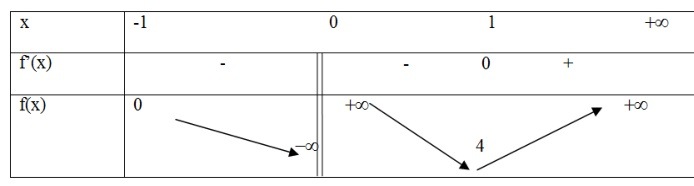
\includegraphics[scale =0.7]{detkl45}
\end{center}
Dựa vào bảng biến thiên, phương trình có nghiệm duy nhất khi và chỉ khi $\left[\begin{matrix}
m<1\\ 
m=4 
\end{matrix}\right]$\\
Dựa vào bảng biến thiên, phương trình có nghiệm duy nhất khi và chỉ khi $[-2017;2017]$.
}
} 
 
  
\baitracnghiem{detk2017:b46}{
 Gọi S là tập hợp tất cả các giá trị thực của tham số $m$ để đồ thị của hàm số $y=\dfrac{1}{3}x^3-mx^2+(m^2-1)x$ có hai điểm cực trị là $A$ và  $B$ sao cho $A, B$ nằm khác phía và cách đều đường
thẳng  $y=5x-9$. Tính tổng tất cả các phần tử của $S$.
}{ 
\datcot\bonpa
{\dung{$0$.}}
{\sai{$6$.}}
{\sai{$-6$.}}
{\sai{$3$.}}
\loigiai{
Ta có $y'=x^2-2mx+m^2, y'=0\Leftrightarrow x=m-1,x=m+1$.\\
Đồ thị hàm số luôn có hai điểm cực trị 
$A\left(m-1;\dfrac{1}{3}(m-1)^2(m+2)\right)$ và
$A\left(m+1;\dfrac{1}{3}(m+1)^2(m-2)\right)$.\\
Trung điểm  $I$ của  $AB$ có tọa độ:  $I\left(m;\dfrac{m^3-3m}{3}\right)$.
Yêu cầu đề bài thỏa mãn khi và chỉ khi  $I$ thuộc đường thẳng $y=5x-9$, hay
$$\dfrac{m^3-3m}{3}=5m-0\Leftrightarrow m^3-18m+27=0.$$
Suy ra tổng các phần tử của  $S$ bằng  $0$ . Chọn \dapandung.
}
} 
 
  
\baitracnghiem{detk2017:b47}{
Trong không gian với hệ tọa độ $Oxyz$ cho mặt phẳng $(P): x-2y+2z-3=0$ và mặt cầu $(S):x^2+y^2+z^2+2x-4y-2z+5=0$.
Giả sử điểm $M\in (P)$ và $N\in (S)$ sao cho vectơ $\overrightarrow{MN}$ cùng phương
với vectơ  $\vec u(1;0;1)$ và khoảng cách giữa  $M$ và  $N$ lớn nhất. Tính  $MN$. 
}{ 
\datcot\bonpa
{\sai{$MN=3$.}}
{\dung{$MN=1+2\sqrt2$.}}
{\sai{$MN=3\sqrt2$.}}
{\sai{$MN=14$.}}
\loigiai{
Mặt cầu $(S):(x+1)^2+(y-2)^2+(z-1)^2=1$, có tâm $I(-1;2;1)$ và bán kính $R=1$.
Gọi  $\Delta$ là đường thẳng đi qua  $I$ và có vectơ chỉ phương $\vec u=(1;0;1)$, khi đó $\Delta:\begin{cases}
x&=-1+t\\
y&=2\\
z&=1+t
\end{cases}$.\\
Đường thẳng  $\Delta$ cắt $(P)$ tại $M(1;2;3)$.  \\
Đường thẳng  $\Delta$ cắt  $(S)$ tại hai điểm $N_1\left(-1-\dfrac{1}{\sqrt2};2;1-\dfrac{1}{\sqrt2}\right)$,
$N_2\left(-1+\dfrac{1}{\sqrt2};2;1+\dfrac{1}{\sqrt2}\right)$.\\
Ta có $MN_1=2\sqrt2+1, MN_2=2\sqrt2-1$ nên ta có $MN=2\sqrt2+1$. Chọn \dapandung.
}
} 
 
  
\baitracnghiem{detk2017:b48}{
 Xét các số phức $z$ thỏa mãn $|z+2-i|+|z-4-7i|=6\sqrt2$.  Gọi $m,M$ lần lượt là giá trị nhỏ nhất, giá
trị lớn nhất của  $|z-1+i|$. Tính  $P=m+M$.
}{ 
\datcot[2]\bonpa
{\sai{$P=\sqrt{13}+\sqrt{73}$.}}
{\dung{$P=\dfrac{5\sqrt{2}+2\sqrt{73}}{2}$.}}
{\sai{$P=5\sqrt{2}+\sqrt{73}$.}}
{\sai{$P=\dfrac{5\sqrt{2}+\sqrt{73}}{2}$.}}
\loigiai{
Gọi  $M$ là điểm biểu diễn số phức  $z$, $F_1(-2;1),F_2(4;7)$ và $N(1;-1)$.\\
Từ $|z+2-i|+|z-4-7i|=6\sqrt2$ và $F_1F_2=6\sqrt2$ nên ta có  $M$ là đoạn thẳng $F_1F_2$. Gọi $H$ là hình chiếu của  $N$ lên $F_1F_2$, ta có $H\left(-\dfrac{3}{2};\dfrac{3}{2}\right)$.\\
Suy ra $P=NH+NF_2=\dfrac{5\sqrt2+2\sqrt{73}}{2}$. Chọn \dapandung.
}
} 
 
  
\baitracnghiem{detk2017:b49}{
 Cho mặt cầu tâm $O$, bán kính $R$. Xét mặt phẳng $(P)$ thay đổi cắt mặt cầu theo giao tuyến là đường
tròn $(C)$. Hình nón $(N)$ có đỉnh $S$ nằm trên mặt cầu, có đáy là đường tròn $(C)$ và có chiều cao là $h (h>R)$.
Tính h để thể tích khối nón được tạo nên bởi $(N)$ có giá trị lớn nhất.
}{ 
\datcot\bonpa
{\sai{$h=\sqrt3 R$.}}
{\sai{$h=\sqrt2 R$.}}
{\dung{$h=\dfrac{4R}{3}$.}}
{\sai{$h=\dfrac{3R}{2}$.}}
\loigiai{
Gọi  $I$ là tâm mặt cầu và  $H$,  $r$ là tâm và bán kính của $(C)$.\\
Ta có $IH=h-R$ và $r^2=R^2-IH^2=2Rh-h^2$.\\
Thể tích khối nón $V=\dfrac{1}{3}\pi r^2 h=\dfrac{\pi}{3}h(2Rh-h^2)=\dfrac{\pi}{3}h.h.(2R-h)$.\\
Ta có $h.h.(4R-2h)\le \left(\dfrac{h+h+4R-2h}{3}\right)^3=\left(\dfrac{4R}{3}\right)^3\Rightarrow h^2(2R-h)\le \dfrac{1}{2}\left(\dfrac{4R}{3}\right)^3.$\\
Do đó  $V$ lớn nhất khi $h=4R-2h\Leftrightarrow h=\dfrac{4R}{3}$. Chọn \dapandung.
}
} 
 
  
\baitracnghiem{detk2017:b50}{
 Cho khối tứ diện có thể tích bằng  $V$. Gọi $V'$ là thể tích của khối đa diện có các đỉnh là các trung
điểm của các cạnh của khối tứ diện đã cho, tính tỉ số $\dfrac{V'}{V}$.
}{ 
\datcot\bonpa
{\dung{$\dfrac{V'}{V}=\dfrac{1}{2}$.}}
{\sai{$\dfrac{V'}{V}=\dfrac{1}{4}$.}}
{\sai{$\dfrac{V'}{V}=\dfrac{2}{3}$.}}
{\sai{$\dfrac{V'}{V}=\dfrac{5}{8}$.}}
\loigiai{
\textbf{Cách 1.} 
\begin{window}[0,r,{
\parbox[t]{\linewidth/3}{\centering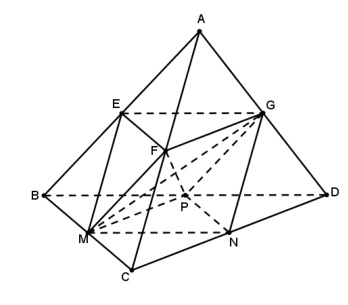
\includegraphics[scale=0.6]{detkl50a}}},]
Ta có $V'=2V_{N.MPGF}=2.2V_{N.MPG}=4V_{G.MNP}=4.\dfrac{1}{2}.\dfrac{1}{4}V_{ABCD}=\dfrac{1}{2}V.$
(Do $G$ là trung điểm $AD, S_{MNP}=\dfrac{1}{4}S_{BCD}$). Do đó $\dfrac{V'}{V}=\dfrac{1}{2}$.
\vspace*{2cm}
\end{window}
\textbf{Cách 2.}
\begin{window}[0,r,{\hspace*{1cm}
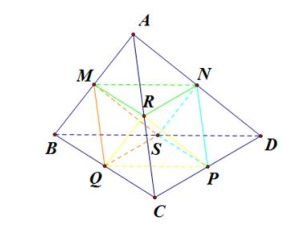
\includegraphics[scale=0.8]{detkl50b}},]
Gọi $M,N,P,Q,R,S$ thứ tự là trung điểm các cạnh
$AB,AD,CD,CB,AC,BD.$\\
Xét $\dfrac{V_{A.MNR}}{V_{A.BCD}}=\dfrac{AM.AN.AR}{AB.AD.AC}=\dfrac{1}{2}.\dfrac{1}{2}.\dfrac{1}{2}=\dfrac{1}{8}$. Hay $V_{A.MNR}=\dfrac{1}{8}V$,
\end{window}
Tương tự $V_{B.MQR}=V_{C.PQR}=V_{D.NPR}=\dfrac{1}{8}V$.\\
Suy ra $V'=V-4.\dfrac{1}{8}V=\dfrac{V}{2}\Rightarrow \dfrac{V'}{V}=\dfrac{1}{2}$.
}
} 
 
%%%%Lấy bảng mã%%%%%%%%%%%%%
% \soanma

\end{document}

